\documentclass[a4paper,11pt]{article} %article style with 11pt fontsize
\usepackage[utf8]{inputenc} %to add symbols like accents
\usepackage{graphicx} % to add figures
\usepackage{amsmath} % to add math and equation environments
\usepackage[margin=3cm]{geometry} % to define the style of the page, margin of 3cm
\usepackage{multicol} %you might need to do multiple columns
\usepackage{hyperref} %to create hyperlinks within the document

\renewcommand{\contentsname}{Table of Contents} %renewcommand is used to be able to name your Table of Contents as you want, default is 'Contents'. Renewcommand with \contentsname allows you to do that. 

\begin{document}

\begin{titlepage}
\begin{center}
\title{YOUR UNIVERSITY}
\large\underline{YOUR FACULTY} 
\par \vspace{0.4in} %\vspace can give you a set vertical space (in inches 'in' or centimeters 'cm') between the previous and following lines to this command
\normalsize{Volume 1 of 1}
\par \vspace{0.4in}
\large{\textbf{YOUR THESIS TITLE}}
\par \vspace{0.2in}
{by}
\par \vspace{0.2in}
\large{\textbf{YOUR NAME}}
\par \vspace{0.4in}
\large{Thesis for the degree of Doctor of Philosophy}
\par \vspace{0.5in}


\end{center}
\end{titlepage}

\newpage\null\thispagestyle{empty}\newpage %leave the next page as blank
\pagestyle{plain}

\setcounter{secnumdepth}{3} % organisational level that receives a numbers
% Print table of contents for level 3
% Levels are: 0 - chapter, 1 - section, 2 - subsection, 3 - subsubsection
\setcounter{tocdepth}{3}  % toc = table of contents, latex uses that abbreviation
\pagenumbering{roman} % roman style (page numbering) for the table of contents

\addcontentsline{toc}{section}{\Large{\textbf{Table of Contents}}} %we are adding an entry to TOC, which is TOC! We want TOC to be listed in the list.
\tableofcontents 
\cleardoublepage % this command ends the current page
\pagenumbering{arabic} % arabic style (page numbering) for the rest of the document
\include{Abstract} 
\include{Intro}
\include{Method}
\include{Conclusions}

\section{Supplementary Information}
\label{sec:conc}
\begin{figure}[h!]
  \caption{ Intercomparison of ${\Delta^{14}CO_{2}}$ measurements  at Cape Grim, Tasmania (CGO), and Baring Head, New Zealand (BHD) collected by NIWA and measured at Rafter Radiocarbon Laboratory. Dates represent the middle of the sampling period, which differ no more than one day between sites. These data show that during the time in which data are available, no measureable difference is found between the two sites. This provides some evidence that the two sites may be considered equivalent for this intercomparability study.}
% This data originally was sent to me in Jocelyn's first dropbox file. Later it was condensed to the currnent file in the H: drive.  H:\Science\Datasets\CGOvBHD
  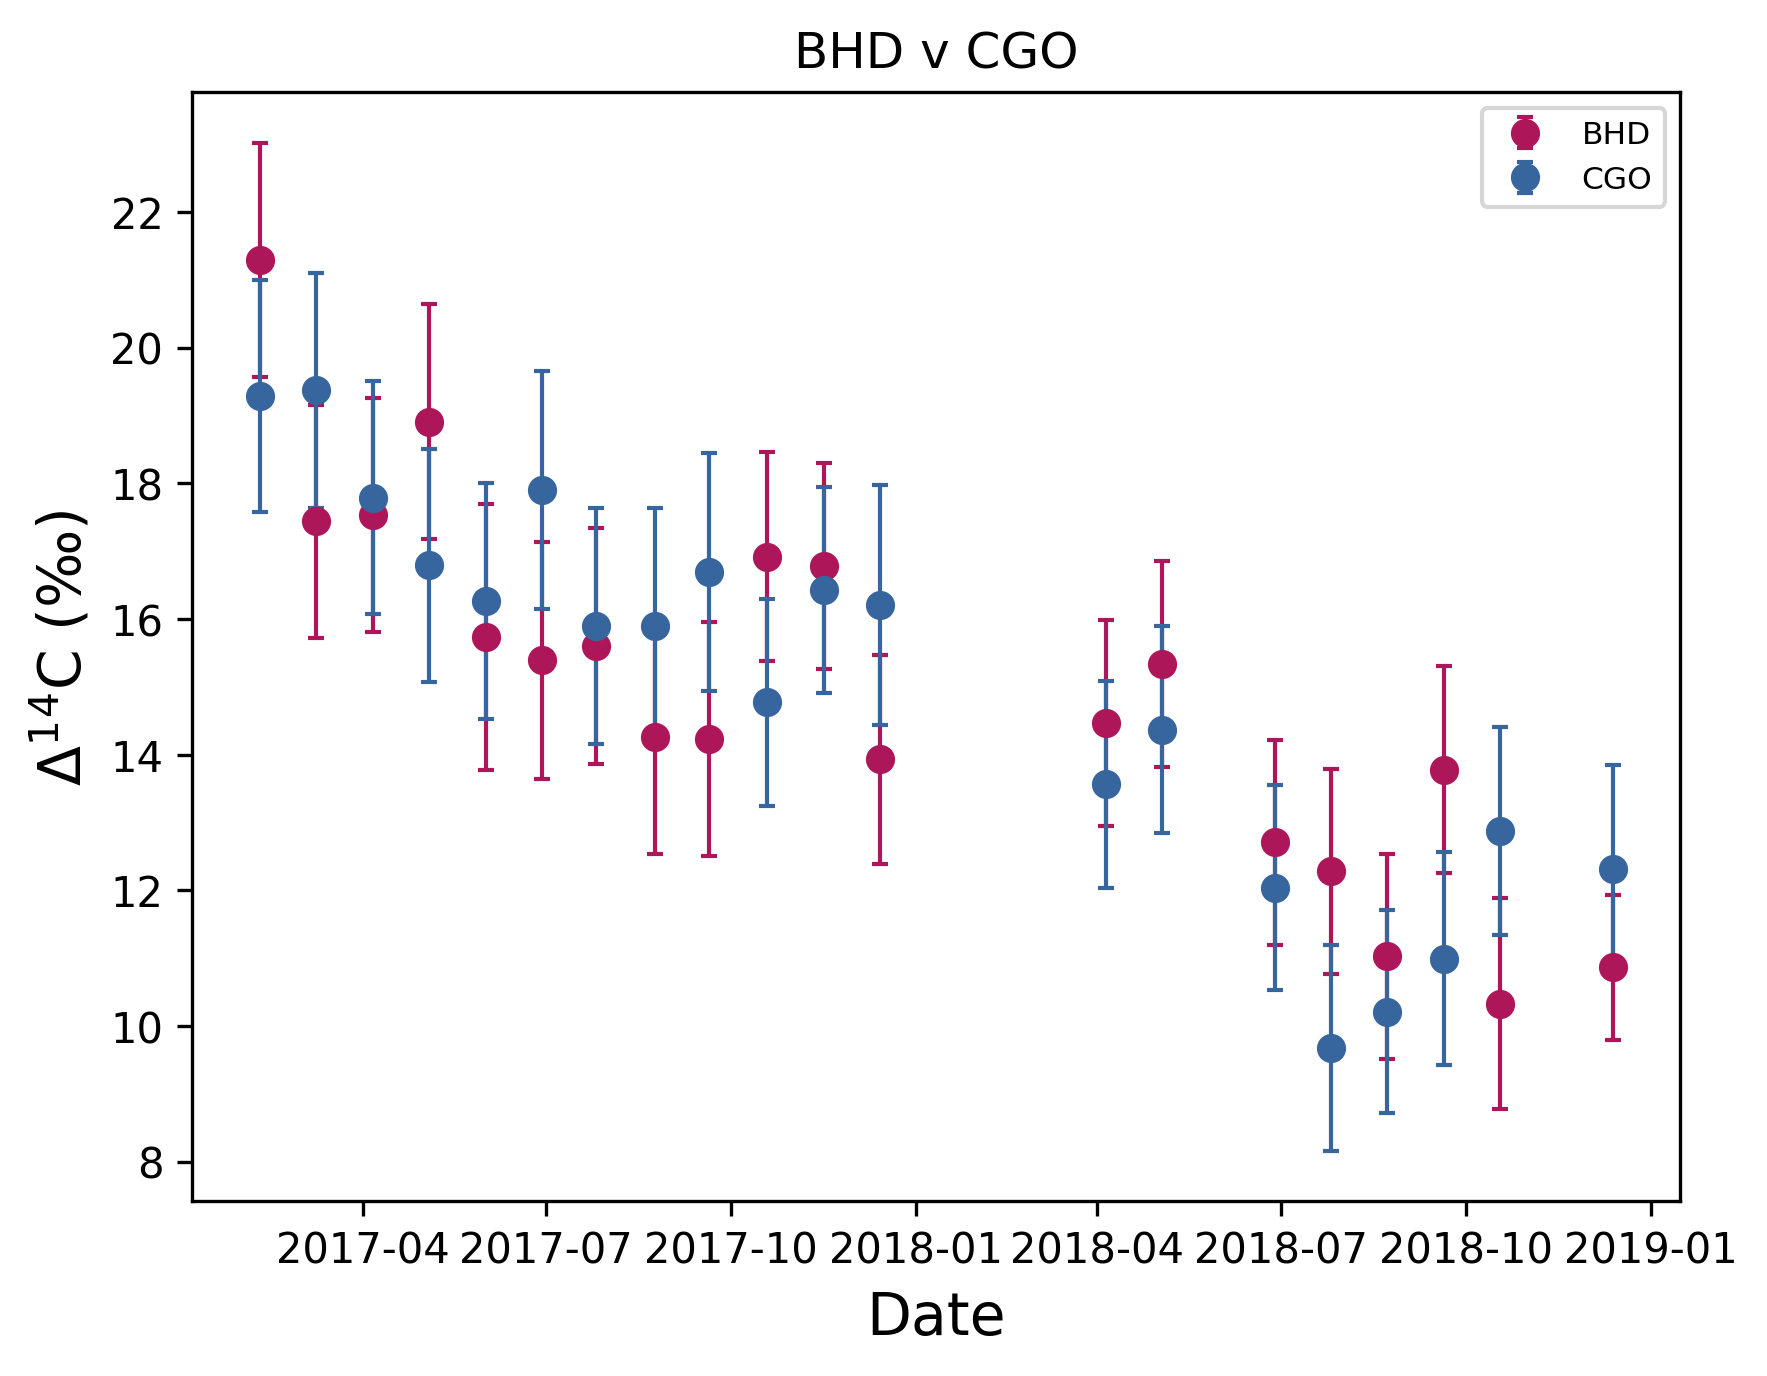
\includegraphics[width=1\textwidth]{/mnt/c/Users/clewis/IdeaProjects/GNS/Interlab_Comparison/output/Site_intercomparison.png}
\label{fig:bhdvcgo}
\end{figure}


\end{document}